\documentclass[border=6pt]{standalone}
%=======================================================================
%  ICCIT 2026 -- CAMERA-READY version, 6 pages, IEEE conference format
%  From Spikes to Sentences: A Hybrid CTC Decoder with Confidence-Gated
%  Language Model Rescoring
%  Compile: pdflatex x3, with revision_results.tex in this folder.
%=======================================================================

\usepackage{amsmath,amssymb}
\usepackage{graphicx}
\usepackage{booktabs}
\usepackage{multirow}
\usepackage{array}
\usepackage{xcolor}
\usepackage{tikz}
\usetikzlibrary{arrows.meta,positioning,calc,fit,backgrounds,shapes.geometric}
\usepackage{pgfplots}
\pgfplotsset{compat=1.17}
\usepackage{algorithm}
\usepackage{algpseudocode}
\usepackage{adjustbox}



\definecolor{ioFill}{HTML}{ECEFF4}\definecolor{ioLine}{HTML}{4C566A}
\definecolor{acFill}{HTML}{E3EEF9}\definecolor{acLine}{HTML}{3B6EA5}
\definecolor{reFill}{HTML}{E0F0EC}\definecolor{reLine}{HTML}{2E8B7F}
\definecolor{trFill}{HTML}{ECE6F5}\definecolor{trLine}{HTML}{6A4C93}
\definecolor{deFill}{HTML}{E6F0E1}\definecolor{deLine}{HTML}{4E8B3B}
\definecolor{llFill}{HTML}{FBEBDD}\definecolor{llLine}{HTML}{C1662F}
\definecolor{gaFill}{HTML}{FFF6E9}\definecolor{gaLine}{HTML}{B8860B}
\definecolor{inkLine}{HTML}{3B4252}

\tikzset{
  blk/.style={rounded corners=3pt,draw,line width=0.9pt,align=center,
              inner sep=4pt,font=\footnotesize},
  io/.style={blk,fill=ioFill,draw=ioLine},
  ac/.style={blk,fill=acFill,draw=acLine},
  re/.style={blk,fill=reFill,draw=reLine},
  tr/.style={blk,fill=trFill,draw=trLine},
  de/.style={blk,fill=deFill,draw=deLine},
  ll/.style={blk,fill=llFill,draw=llLine},
  gate/.style={diamond,aspect=1.7,draw=gaLine,fill=gaFill,line width=0.9pt,
               align=center,inner sep=1pt,font=\footnotesize},
  fl/.style={-{Stealth[length=5pt]},line width=0.9pt,draw=inkLine},
  dec/.style={-{Stealth[length=5pt]},line width=0.8pt,draw=deLine,dashed},
  tag/.style={font=\scriptsize\itshape,text=inkLine,fill=white,inner sep=1pt},
  capt/.style={font=\scriptsize,text=ioLine},
}

\newcommand{\pct}{\,\%}


\begin{document}
\setlength{\columnwidth}{3.5in}
\fontsize{10}{12}\selectfont
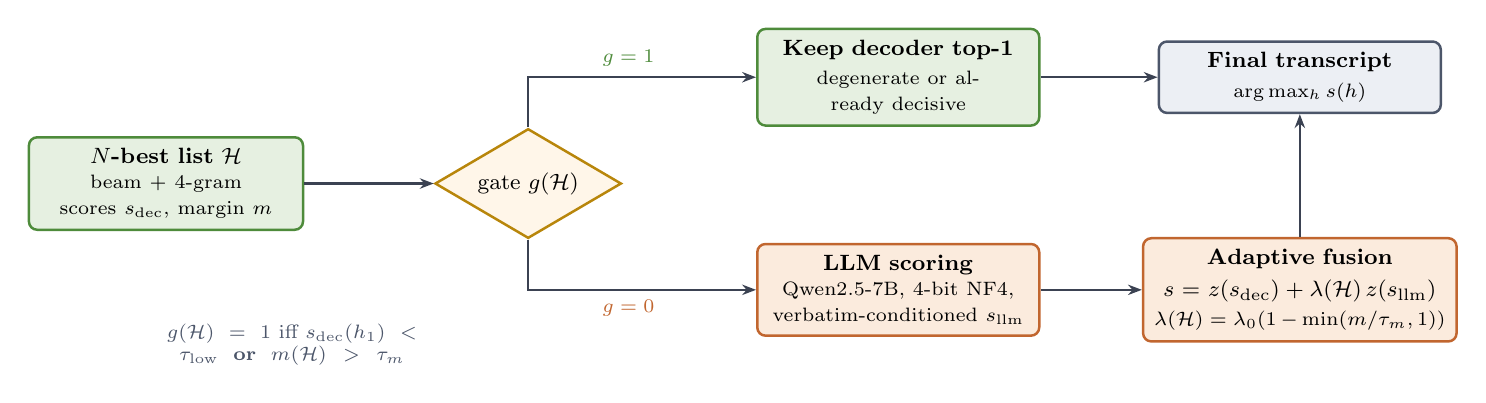
\begin{tikzpicture}[every node/.style={font=\footnotesize}]
  \node[de,text width=32mm] (nb) at (0,0)
       {\textbf{$N$-best list $\mathcal{H}$}\\[1pt]\scriptsize beam $+$ 4-gram\\ scores $s_{\mathrm{dec}}$, margin $m$};
  \node[gate,text width=17mm] (g) at (4.6,0) {gate $g(\mathcal{H})$};
  \node[de,text width=33mm] (keep)  at (9.3,1.35)
       {\textbf{Keep decoder top-1}\\[1pt]\scriptsize degenerate or already decisive};
  \node[ll,text width=33mm] (score) at (9.3,-1.35)
       {\textbf{LLM scoring}\\[1pt]\scriptsize Qwen2.5-7B, 4-bit NF4,\\ verbatim-conditioned $s_{\mathrm{llm}}$};
  \node[ll,text width=37mm] (fuse) at (14.4,-1.35)
       {\textbf{Adaptive fusion}\\[2pt]
        $s=z(s_{\mathrm{dec}})+\lambda(\mathcal{H})\,z(s_{\mathrm{llm}})$\\[1pt]
        \scriptsize $\lambda(\mathcal{H})=\lambda_0(1-\min(m/\tau_m,1))$};
  \node[io,text width=33mm] (out) at (14.4,1.35)
       {\textbf{Final transcript}\\[1pt]\scriptsize $\arg\max_h s(h)$};

  \draw[fl] (nb) -- (g);
  \draw[fl] (g) |- node[capt,pos=0.72,above,text=deLine]{$g=1$} (keep);
  \draw[fl] (g) |- node[capt,pos=0.72,below,text=llLine]{$g=0$} (score);
  \draw[fl] (score) -- (fuse);
  \draw[fl] (fuse) -- (out);
  \draw[fl] (keep) -- (out);

  \node[capt,text width=46mm,align=center] at (1.6,-2.05)
       {$g(\mathcal{H})=1$ iff $s_{\mathrm{dec}}(h_1)<\tau_{\mathrm{low}}$ \textbf{ or } $m(\mathcal{H})>\tau_m$};
\end{tikzpicture}
\end{document}
